\documentclass[runningheads]{llncs}
\usepackage{amssymb}
\setcounter{tocdepth}{3}
\usepackage{graphicx,epsfig}
\usepackage{algorithmic}
\usepackage{listings}
\usepackage{rotating}
\usepackage{subfig}

%%%%

\usepackage{color}
\usepackage{alltt}
\usepackage{verbatim}
\usepackage{url}
\usepackage[utf8]{inputenc}
\usepackage[spanish]{babel}

%%

\usepackage{url}
%\urldef{\mailsa}\path|pgarcia@atc.ugr.es|

\urldef{\mailsa}\path|pgarcia@atc.ugr.es|

\newcommand{\keywords}[1]{\par\addvspace\baselineskip
\noindent\keywordname\enspace\ignorespaces#1}

\lstset{
basicstyle=\ttfamily \scriptsize,
language=c++,
frame=single,
stringstyle=\ttfamily,
showstringspaces=false
}

\renewcommand{\textfraction}{0}
\renewcommand{\topfraction}{1}
\renewcommand{\bottomfraction}{1}
\renewcommand{\floatpagefraction}{0.9}

\begin{document}

\mainmatter  % start of an individual contribution



% first the title is needed
\title{Desarrollo de servicios para una Arquitectura Orientada a Servicios para Algoritmos Evolutivos \thanks{Este trabajo ha sido desarrollado bajo los proyectos EvOrq (TIC-3903), CEI BioTIC GENIL (CEB09-0010), MICINN CEI Program (PYR-2010-13) and FPU research grant AP2009-2942 .
}}


% a short form should be given in case it is too long for the running head
\titlerunning{Desarrollo de servicios para una Arquitectura Orientada a Servicios para Algoritmos Evolutivos}
%\author{No author given}
\author{P. Garc\'ia-S\'anchez\inst{1}, A. E. Eiben\inst{2}, E. Haasdijk\inst{2}, B. Weel\inst{2} and J.J. Merelo\inst{1}}

%

\authorrunning{P. Garc\'ia-S\'anchez et al.}
%\authorrunning{Anonymous.}
% (feature abused for this document to repeat the title also on left hand pages)
% the affiliations are given next; don't give your e-mail address
% unless you accept that it will be published

\institute{Dept. of Computer Architecture and Technology, University of Granada, Spain \and Dept. of Computer Science, Vrije Universiteit Amsterdam, The Netherlands
\mailsa}
%\institute{No institute given
%\mailsa}




%\toctitle{BLABLABLA}

%\tocauthor{Authors' Instructions}
\maketitle


\begin{abstract}
We investigate on-line on-board evolution of robot controllers based
on the so-called hybrid approach (island-based). Inherently to this approach each
robot hosts a population (island) of evolving controllers and
exchanges controllers with other robots at certain times. We compare
different exchange (migration) policies in order to optimize this
evolutionary system and compare the best hybrid setup with the
encapsulated and distributed alternatives. We conclude that adding a difference-based migrant
 selection scheme increases the performance.
%Not too clear now. You don't define hybrid , and what I understand
%here is that you optimize something and you compare it with something
%else, but it's not clear what conclusion you obtain from the
%optimization and why do you compare it. Is it better? Worse? - JJ
%Pablo: added "(island-based)" and conclusions in the abstract
 
%This work presents the results obtained from comparing several migration policies that tries to optimize in a noisy fitness environment: the on-line, on-board and hybrid evolutionary robotics problem. Three different migration policies have been studied (the most different migrant, random migrant and best migrant) and two replacement mechanisms: the migrant replaces the worst, or the migrant replaces the worst after being evaluated only if is better. Experiments with 4, 16 and 36 robots were conduced, with two different topologies (ring and panmictic) and also a comparison with other evolutionary robotics algorithms were performed. Results show that the replacement mechanism has more influence than the migration policy or topology, and it also affects the tuning of the algorithm parameters.

% You should conclude something about the
            % "multiculturality" of the algorithm and explain results
            % via diversity - JJ

\end{abstract}

\section{Introduction}
\noindent Service Oriented Architecture (SOA) \cite{PAPAZOGLOU} se está convirtiendo en un importante TREND en el desarrollo de software. Este paradigma permite la organización y distribución utilizando el concepto de {\em servicio}. Un servicio es la interacción mostrada en la figura \ref{SOADIAGRAM}. El {\em proveedor de servicio} publica {\em descripciones de servicio} (o interfaces) en el {\em registro de servicios}, para que los {\em consumidores de servicio} puedan encontrarlo y enlazarse con los proveedores de servicio para usarlo.

SOA permite independencia en el lenguaje de programación y los mecanismos de distribución, centrándose en la extensión e integración fáciles, pero cuenta con las siguientes restricciones:

\begin{itemize}
\item Los servicios deben ser funciones de entrada/salida.
\item Los servicios no deben tener estado (es decir, no usar variables globales).
\item El orden de ejecución de los servicios no es fijo.
\item Los servicios deben ser diseñados tan abstractos como sea posible.
\end{itemize}

La computación distribuida ofrece la posibilidad de utilizar las ventajas del procesamiento paralelo y así conseguir un mayor poder de cómputo \cite{OPENSCIENCEGRID}.
SOA también puede aplicarse a este área, utilizando plataformas basadas en Web Services \cite{PAPAZOGLOU}, o nuevos estándars para este paradgima, como OSGi (Open Services Gateway Initiative) \cite{OSGI}.

OSGi permite construir sistemas software de calidad considerando un alto nivel de modularidad. Aparte de los beneficios que los paradigmas clásicos de modularización ofrecen (como el modelado orientado a objetos) y las mejoras en testeo, reusabilidad, disponibilidad y mantenibilidad, es necesario explorar otras técnicas, como el desarrollo basado en plug-ins o el diseño SOA. Este tipo de desarrollo simplifica aspectos como la complejidad, personalización, configuración, y coste del desarrollo. En el campo de las heurísticas de optimización los beneficios the usar este tipo de desarrollo tienen lugar en el desarrollo de algorithmos, evaluación experimental y combinación de diferentes paradigmas de optimización \cite{PLUGINS}.

%\begin{figure}[ht] 
%\begin{center} 
 % \epsfig{file=soaDiagram.eps,width=7.5cm} 
%\includegraphics[scale=1]{images/soaDiagram.eps}
%\end{center} 
%\caption{Esquema de interacción de servicios. El proveedor de servicios publica una descripción de servicio que es utilizada por el consumidor de servicios para encontrar y usar servicios.} 
%\label{SOADIAGRAM} 
%\end{figure} 

En nuestro trabajo anterior \cite{OSGILIATH} presentamos una Arquitectura Orientada a Servicios para Algoritmos Evolutivos (SOA-EA), junto con guías y pasos para migrar del desarrollo tradicional de Algoritmos Evolutivos (AEs) a SOA. También presentó una implementación específica, llamada OSGiLiath ({\em OSGi Laboratory for Implementation and Testing of Heuristics}): un entorno para el desarrollo de algoritmos distribuidos extensible con una arquitectura basada en plug-ins y basada en una especificación software ampliamente aceptada (OSGi). En este trabajo presentamos el desarrollo completo de un servicio utilizando la tecnología específica, en lugar del diseño abstracto presentado en nuestro anterior trabajo.

El resto del trabajo se estructura como sigue: después del estado del arte, presentamos los principios de diseño para crear servicios para Computación Evolutiva (CE) (Sección \ref{sec:design}). A continuación, se explica la tecnología de implementación OSGi en la Sección \ref{sec:technology}, utilizada para construir nuestro framework (descrito en la Sección \ref{sec:osgiliath}). Después, los pasos para crear servicios dentro de este framework se presentan (Sección \ref{sec:development}). Finalmente se presentan las conclusiones y trabajo futuro (Sección \ref{sec:conclusions}).



\section{Estado del arte}
\label{sec:soa}

Aunque SOA se usa ampliamente en el desarrollo de software no está muy aceptada en la comunidad de las metaheurísticas. La mayoría de los frameworks tienen carencia de la baja generalidad, ya que están enfocados en un campo específico, como EasyLocal++ \cite{EASYLOCAL}(centrado en Búsqueda Local) o SIGMA \cite{SIGMA} (en el campo de optimización de sistemas de soporte  a la decisión). Otro problema común es que suelen ser simplemente librerías o múdulos Perl \cite{PERL}, no tienen GUIs o son muy complicados de instalar y requieren muchas destrezas de programación. Otro problema puede ser la pérdida de confort a la hora de programar, por ejemplo, C tiene una sintaxis más complicada que otros lenguajes.

Entre la gran cantidad de herramientas software que existen, queremos centrarnos en los frameworks de algoritmos distribuídos más aceptados. ECJ \cite{ECJ}, Evolutionary Computation in Java, es un conjunto de clases Java que pueden ser extendidas e incluyen varios módulos de comunicación. MALLBA \cite{MALLBA} se basa en esqueletos software con una interfaz común pública. Cada esqueleto implementa una técnica de resolución para optimizaciónen el campo de optimización exacta, heurística o híbrida. Proporciona capacidades de distribución utilizando MPI. Sin embargo estos dos frameworks no se basan en el desarrollo orientado a plug-ins, por lo que no pueden tomar las ventajas de características como gestión del ciclo de vida, versionado o enlazado dinámico de servicios, como propone OSGi.

Otra plataforma importante es DREAM \cite{DREAM}, un framework open source para Algoritmos Evolutivos basado en Java que define un modelo de isla y usa el protocolo Gossip y sockets TCP/IP para comunicación. Puede desplegarse en plataformas P2P y está dividido en cinco capas. Cada capa proporciona una interfaz de usuario y diferentesniveles de interacción y abstracción, pero añadir nuevas funcionalidades no es tan fácil, debido al hecho de que el sistema debe pararse antes de añadir nuevos módulos y la implementación de interfaces debe estar definida en el código fuente, por lo que necesita compilarse con cada elemento a añadir (como en ECJ). OSGi permite añadir nuevas funcionalidades sólamente compilando las nuevas características y no ya las existentes.

Among this great number of software tools we want to focus in the most widely accepted distributed algorithms frameworks. ECJ \cite{ECJ}, Evolutionary Computation in Java, is a set of Java classes that can be extended and includes several communication modules. MALLBA \cite{MALLBA} is based in software skelletons with a common and public interface. Every skeleton implements a resolution technique for optimization in the fields of exact, heuristic or hybrid optimization. It provides LAN and WAN capacity distribution with MPI . However, this both frameworks are not based in the plug-in development, so they can not take advantage of features like the life-cycle management, versioning, or dynamic service binding, as OSGi proposes.

Los autores de MALLBA están trabajando ahora en el framework jMetal \cite{JMETAL}, un nuevo framework basado en Java, pero sin posibilidad de distribución y mayormente centrado en optimización Multi-Objetivo.

ParadiseEO \cite{PARADISEO} permite el diseño de AEs y Búsqueda Local con hibridación, proporcionando una gran variedad de operadores y funciones de evaluación. También implementa los modelos paralelos y distribuídos más comunes, y está basado en librerías estándar como MPI, PVM y Pthreads. Sin embargo, cuenta con los mismos problemas que los frameworks anteriores, no cuenta con gestión del ciclo de vida, ni programación orientada a servicios. GAlib \cite{GALIB} es muy similar y comparte las mismas características y problemas. 

En el campo de los frameworks basados en plug-ins, HeuristicLab \cite{HEURISTICLAB} es el ejemplo más avanzado. Permite además programación distribuída utilizando Servicios Web y una base de datos centralizada, pero no usa su propio diseño de plug-ins para la comunicación distribuída.


METCO  \cite{METCO} cuenta con los mismos problemas que los frameworks anteriores, no utiliza un sistema de plug-ins estándar ni SOA, pero permite la implementación de interfaces existentes y configurar sus funcionalidades. 

Finalmente, el único framework orientado a servicios para optimización es GridUFO \cite{GRIDUFO}, pero sólo permite la modificación de la función objetivo y añadir nuevos algoritmos, sin poder combinar servicios existentes.

Los frameworks anteriores han sido diseñados para ser extendibles y re-usables, pero sin tener en cuenta las restricciones de SOA para lograr más independencia y mejoras en el desarrollo.

\section{Diseñando servicios para una Arquitectura Orientada a Servicios para AEs}
\label{sec:design}

En \cite{OSGILIATH} demostramos que es posible crear una arquitectura orientada a servicios para AEs utilizando una tecnología SOA específica. Esta arquitectura utiliza las capacidades que SOA ofrece. Para hacer esto, se desarrollaron servicios débilmente acoplados para EAs (SOA-EA), y se implementarion utilizando una tecnología SOA y se compararon con otros frameworks. Estos servicios pueden combinarse de varias formas para obtener diferentes algoritmos (por ejemplo, de un AG canónico se puede crear un NSGA-II simplemente añadiendo nuevos servicios). También se presentaron varias técnicas para combinar servicios de forma flexible.


\subsection{Principios de diseño}

Una de las restricciones principales de SOA, además de el enfoque en servicios abstractos es la naturaleza sin estado de los servicios. Por lo tanto, en SOA el diseño de servicios debe seguir varias GUIDELINES?

Para empezar, debido a que los servicios no tienen por qué tener conocimiento de otros servicios, no debe haber variables globales en ninguna parte del código. Los servicios están escuchando y esperando a ser ejecutados. Por ejemplo, debe evitarse una función fitness con un contador que se incremente cada vez que se llama (para parar el algoritmo al llegar a un límite). Si varios (y diferentes) algoritmos están trabajando en paralelo, a la vez, y llamando a esta función a la vez el contador no distinguiría entre algoritmos, ofreciendo resultado erróneos. Sin embar, un servicio que mantiene algún tipo de estado se permite, por ejemplo, un servicio de estadísticas que lee eventos de todos los algoritmos que se ejecutan a la vez, pero debe ser administrado para evitar errores.

Además, un servicio debe ser indistinguible de ser ejecutado de forma local o remota en otro nodo de la red. Cada etapa del algoritmo debe ser tratada como servicio a ser ejecutado en local o en remoto, incluso un servicio de {\em Población} o {\em Parámetros}. Deben proveerse mecanismos correctos para el intercambio de datos. Incluso muchas implementaciones del mismo servicio pueden existir a la vez (por ejemplo, diferentes implementaciones del servicio {\em Crossover}), y deberían ser manejados y usados corrrectamente.

Un servicio es siempre una función solicitud-respuesta. Por ejemplo, el cálculo del fitness no debe ser un método de la implementación {\em Individuo}, si no una función que recibe una lista de individuos y devuelve una lista de fitness de esos individuos. Esto permite opciones como cálculo remoto del fitness y balanceo de carga distribuído, imposible de realizar si el fitness es un método de la clase Individuo.

Pensando lo más abstractamente posible requiere separar conceptos como el orden de recombinación, y el propio crossover. Normalmente, después de la selección de los padres, los individuos se cruzan en orden. Sin embargo, si necesitamos un mecanismo de emparejamiento distinto (por ejemplo, usar más de un padre, o seleccionar un padre más de dos veces) se necesita una duplicación de esfuerzo. Esta es la razón por la que se deben separar conceptoos como {\em recombinación} de {\em crossover}. 

Finalmente, no debemos asumir sobre el orden de los servicios a ejecutar. Por ejemplo, servicios como {\em Recombinador} or {\em Mutator} deberían devolver los individuos con el fitness ya calculado. Normalmente este paso se realiza en la última etapa de la generación, pero podría ser necesario obtenerlo anteriormente para ser usados en otras tareas, por ejemplo una búsqueda local o un recolector de estadísticas para guiar al algoritmo.

\subsection{Otras restricciones tecnológicas}

En \cite{OSGILIATH} presentamos las ventajas de usar SOA en algoritmos Evolutivos: para empezar, SOA encaja con las ventajas de generalidad en el desarrollo de AEs explicado en \cite{GENERICITY05}, pero añade nuevas características, como independencia del lenguaje y mecanismos de distribución. También permite añadir y eliminar servicios en tiempo de ejecución sin alterar la ejecución general del algoritmo (esto, no es obligatorio pararlo o añadir código extra para soportar nuevos operadores). Esto permite incrementar la interoperabilidad entre diferentes elementos software. Además, esto permite distribución del código de manera fácil: SOA no requiere de una implementación o librería de distribución concreta.

En este trabajo se presenta un proceso de desarrollo, centrado en la tecnología utilizada. Estos servicios deben cumplir las siguientes restricciones tecnológicas:
\begin{itemize}
\item Estos servicios pueden ser enlazados dinámicamente para cambiar los aspectos necesarios del AE.
\item El código fuente de los servicios básico no debe ser reescrito o recompilado para conseguir esta tarea.
\item Nuevos servicios pueden añadirse en tiempo de ejecución.
\item No hace falta código fuente específico para distribución, ni el código fuente de los servicio debe modificarse para este propósito. Es decir, cambiar las librerías de distribución no debe añadir código extra en los servicios existentes.
\end{itemize}

\section{Desarrollo de servicios en OSGiLiath}
\label{sec:development}

Esta sección presenta los pasos para añadir servicios al núcleo de OSGiLiath. En esta sección se explica cómo añadir el problema del Vehicle Routing Problem (VRP).
This section presents the steps to add services to the existent OSGiLiath core. In this section the implementation to add the Vehicle Routing Problem (VRP) are explained.

\subsection{Creación de un bundle}

En OSGiLiath, los servicios se pueden añadir a bundles existentes o crear nuevos. Cada bundle incluye un fichero MANIFEST.MF (como se muestra en la Figura \ref{fig:manifest}). En este caso hemos seleccionado los paquetes que importar (incluyendo interfaces y clases del núcleo de OSGiLiath) y exportar. La sección {\em Service-Description} muestra la localización de Component Definitions para describir los servicios. En este caso se implementan dos interfaces: {\em TransportData} y {\em FitnessCalculator}. Otras clases relacionadas con el VRP se añaden, como {\em Route} o {\em Shop}.


\subsection{Implementando servicios}
Para implementar un servicio se crea una clase que implementa una interfaz. Por ejemplo,  {\em VRPFitnessCalculator} implementa la interfaz {\em FitnessCalculator}. La relación entre estos dos elementos se hace en el Component Definition de la Figura \ref{fig:ds}. De esta forma, la implementación se anuncia a los otros servicios en el entorno, que pueden enlazarse o desenlazarse. Por ejemplo, la implementación {\em VRPInitializer} (implementando {\em Initializer}) requiere esta implementación para crear los individuos. Los servicios pueden enlazarse automáticamente con otros servicios con los métodos set/unset en el Component Definition. Otros servicios fuera del AE pueden añadirse (por ejemplo, en este bundle el servicio {\em TransportData}, que incluye información sobre distancias y tiempo a los nodos). Finalmente, se añaden {\em VRPMutation} and {\em VRPCrossover}siguiendo los consejos proporcionados en la Sección \ref{sec:design}.

\subsection{Añadiendo comunicación}
Gracias a la especificación OSGi 4.2, los servicios pueden y deben ser indistinguibles de los existente

\subsection{Adding communication}
Thanks to the OSGi 4.2 specification, services must be indistinguishable from the ones in the local OSGi environment or in other OSGi environment (in the same machine or even in the same network). To achieve this, the ECF is used to export services. In this case, the {\em Migration} service is used. This service has two operations: send and read. The first one is used to send the individuals to the migrator, and the other is used to read the individuals of that migrator. Usually, each node (island) has one migrator to receive individuals, and references to the other nodes' migrators. In our case, the implementation of {\em Replacer} binds the local {\em Migrator} to write in it the individual(s) to sent. One example of Migrator implementation is the {\em MigratorRingBuffer}: this class implements that interface and automatically binds all the Migrators available in the environment (in a vector of references) thanks to the bind/unbind methods of DS. So, the migrators can be added during runtime, and no stop the algorithm if one node fails.  The {\em MigratorRingBuffer} sends the individuals to the remote Migrator whose id is inmediatelly higher than the local id (a ring). Figure \ref{MIGRATOR} shows this configuration. For example, from the {\em Replacer} implementation, a reference to the local {\em Migrator} interface just send and read the individuasl. The {\em MigratorRingBuffer} implementation binds an unbinds other migrators in other nodes, keeping a reference to these interfaces. Several properties added to the service (for example, in the Figure \ref{fig:ds}) allows to ECF automatically announce the implementation to all nodes in the network and no specific code is required to change from one distribution mechanism to another. 

\section{Conclusiones}
\label{sec:conclusions}
Este trabajo muestra los requisitos para crear un frameowrk orientado a servicios para AEs y la tecnología escogida para cumplir esos requisitos.  Service Oriented Architecture (SOA) ofrece independencia del lenguaje, mecanismos de distribución o incluso sistemas operativos, permitiendo la integración de diferentes elementos. Sin embargo, algunos elementos deben considerarse en el desarrollo: los servicios son funciones de entrada/salida sin estado, los servicios pueden aparecer o desaparecer en tiempo real, y el orden de ejecución no debe estar fijo. En el campo de los AEs los servicios deben desarrollarse teniendo en cuenta estas restricciones. Este trabajo muestra el diseño abstracto de los elementos de un AE, junto con los requisitos tecnológicos a resolver. Se ha utilizado la tecnología OSGi como ejemplo. Los elementos para crear una SOA para AEs han sido presentados junto con un ejemplo de desarrollo.

Como trabajo futuro, se pretende realizar un estudio sobre escalabilidad utilizando otros algoritmos (como GRAS, Scatter Search, Ant Colony Optimization y otros). Además está planeado incrementar el uso de las ventajas de OSGi, como la administración de eventos o la gestión de servicios de forma más profunda. Finalmente, se plantea desarrollar un portal o un repositorio Maven para centralizar todas las implementaciones de problemas y algoritmos para permitir la distribución junto con la plataforma base. También se plantea un estudio sobre portar software existente (especialmente los frameworks escritos en Java, como DREAM o ECJ) a nuestro framework. Además, debido a la facilidad de enlazar implementaciones a interfaces, se plantea desarrollar la funcionalidad de elegir una u otra implementación dependiendo de varios parámetros, o por ejemplo, utilizar Programación Genética para evolucionar e hibridizar algoritmos.

%ACKNOWLEDGMENTS are optional
\section{Acknowledgments}
This work has been supported in part by FPU research grant AP2009-2942 and projects EvOrq (P08-TIC-03903), Project 83 (CANUBE) awarded by the CEI-BioTIC UGR, and TIN2011-28627-C04-02 (ANYSELF).




\bibliographystyle{splncs}
\bibliography{osgiliath}

\end{document}

